% Created 2015-03-21 Sat 04:39
\documentclass[sans,aspectratio=169,presentation,bigger,fleqn]{beamer}
\usepackage[utf8]{inputenc}
\usepackage[T1]{fontenc}
\usepackage{fixltx2e}
\usepackage{graphicx}
\usepackage{longtable}
\usepackage{float}
\usepackage{wrapfig}
\usepackage{rotating}
\usepackage[normalem]{ulem}
\usepackage{amsmath}
\usepackage{textcomp}
\usepackage{marvosym}
\usepackage{wasysym}
\usepackage{amssymb}
\usepackage{capt-of}
\usepackage{hyperref}
\tolerance=1000
\usepackage{setspace}
\setstretch{1.3}
\usepackage{booktabs}
\hypersetup{colorlinks=true,linkcolor=blue,urlcolor=blue}
\usepackage{lmodern}
\usetheme[alternativetitlepage=true,titleline=true]{Torino}
\usecolortheme{freewilly}
\usepackage{lmodern}
\usetheme[alternativetitlepage=true,titleline=true]{Torino}
\usecolortheme{freewilly}
\usetheme{default}
\author{John Henderson}
\date{21 March 2015}
\title{An introduction to \texttt{shiny}}
\begin{document}

\maketitle

\begin{frame}[fragile,label=sec-1]{Why \texttt{R}?}
 Indeed; why in the world subject yourself to:
\begin{itemize}
\item \texttt{<-}
\item \texttt{\%in\%}
\item foo\$bar
\item foo[, "bar"]
\item lists
\item \texttt{lapply()} vs. \texttt{for()}
\end{itemize}
\end{frame}

\begin{frame}[fragile,label=sec-2]{Why \texttt{R}?}
 R is built for statistics and data
\begin{itemize}
\item I picked up \texttt{R} as an alternative to Minitab
\item Cross-platform consistency
\item Great plotting/graphics with \texttt{ggplot()}
\item Incredible data manipulation (\texttt{melt()}, \texttt{ddply()}, subsetting)
\item Huge package repository
\end{itemize}
\end{frame}

\begin{frame}[fragile,label=sec-3]{Why \texttt{R}?}
 But \texttt{R} for interactive web graphics??

\begin{itemize}
\item Requires \textasciitilde{}0 \texttt{html/javascript} knowledge
\item I find it faster to write (e.g. vs. \texttt{d3.js})
\item If you already use \texttt{R}, \texttt{shiny} makes the next step easy
\item Nice for quick prototypes/sketches
\item Exploratory analysis
\end{itemize}
\end{frame}


\begin{frame}[fragile,label=sec-4]{Basics}
 \texttt{shiny} is an \texttt{R} package that enables web based applications
\begin{itemize}
\item Overview of \texttt{shiny} basics
\item Some
\item The code/data necessary to reproduce anything in this talk is on \href{https://github.com/jwhendy/devFest-shiny_2015}{github}
\begin{itemize}
\item \url{https://github.com/jwhendy/devFest-shiny_2015}
\end{itemize}
\end{itemize}
\end{frame}

\begin{frame}[fragile,label=sec-5]{Basics}
 \begin{itemize}
\item You can't do anything in \texttt{shiny} without knowing how to do it in \texttt{R} locally
\item \texttt{shiny} needs to operate inside of \href{http://www.rstudio.com/}{RStudio}
\item\relax [At least] two files are required to run an application
\begin{itemize}
\item \texttt{ui.R}: page format, user inputs, and outputs you're going to create
\item \texttt{server.R}: contains the R code which will generate your dynamic output
\end{itemize}
\end{itemize}

\vspace{0.5cm}

Don't forget to run \texttt{install.packages("shiny")}!
\end{frame}

\begin{frame}[fragile,label=sec-6]{Minimal \texttt{ui.R}}
 \scriptsize
\begin{verbatim}
library(shiny)
# page format
shinyUI(pageWithSidebar(
  # title
  headerPanel("Hello Shiny!"),

  sidebarPanel(
    # user inputs go here
  ),

  mainPanel(
    plotOutput("plot") # what you're going to output, e.g. a plot
  )
))
\end{verbatim}
\scriptsize
\end{frame}

\begin{frame}[fragile,label=sec-7]{Minimal \texttt{server.R}}
 \scriptsize
\begin{verbatim}
library(shiny)

shinyServer(function(input, output) {

  # general R code here: load libraries, set variables/functions/etc.

  # output$name has to match ui.R's plotOutput("name")
  output$plot <- renderPlot({

    # code to make a plot goes here

  })
})
\end{verbatim}
\scriptsize
\end{frame}

\begin{frame}[fragile,label=sec-8]{It works!}
 \begin{itemize}
\item Create the above files\ldots{}
\end{itemize}

\scriptsize
\begin{verbatim}
# run from within R studio
library(shiny)
setwd("/path/to/ui-and-server.R")
runApp()
\end{verbatim}

\begin{center}
\includegraphics[height=3.75cm]{./img/shiny-template.png}
\end{center}
\end{frame}
\begin{frame}[label=sec-9]{Lots of choices}
\begin{columns}
\begin{column}{0.45\columnwidth}
\begin{block}{Input elements}
\begin{itemize}
\item checkbox
\item date (single/range)
\item file upload
\item numeric/text box
\item dropdown
\item slider (single/double)
\end{itemize}
\end{block}
\end{column}

\begin{column}{0.45\columnwidth}
\begin{block}{Output methods}
\begin{itemize}
\item html
\item image
\item plot
\item table
\item text
\item\relax [rendered] markdown
\end{itemize}
\end{block}
\end{column}
\end{columns}
\end{frame}

\begin{frame}[label=sec-10]{Example: data analysis/exploration}
\begin{itemize}
\item Enable rapid and dynamic switching of plot variables
\item Allows for "plot prototyping" to examine trends/relationships
\item Web-based solution is easily sharable with others
\end{itemize}
\end{frame}

\begin{frame}[fragile,label=sec-11]{Fiddling with public transportation data}
 \begin{itemize}
\item Grabbed data on public transportation centers around US (more \href{https://github.com/tcrug/public-transpo}{here})
\item Some are quite efficient, some are horrible
\item Can \texttt{shiny} help find some interesting tidbits?
\end{itemize}

\pause

\href{https://jwhendy.shinyapps.io/transpo-exploration/}{\alert{Demo time!}}
\end{frame}

\begin{frame}[fragile,label=sec-12]{Example: interactive contour plots}
 \begin{itemize}
\item Applied machine learning in \texttt{R} on product test data
\item Contour plots can be nice for visualizing effect of inputs vs. outputs
\item Static plots with lots of inputs/outputs can be cluttered; difficult to show all the
data in one place
\item How to share the results with co-workers who don't use \texttt{R}?
\end{itemize}

\pause

\href{https://jwhendy.shinyapps.io/interactive-contour/}{\alert{Demo time!}}
\end{frame}

\begin{frame}[fragile,label=sec-13]{Example: \texttt{shiny} + \texttt{rCharts}}
 \begin{itemize}
\item \texttt{rCharts} brings an \texttt{R} interface to several existing \texttt{javascript} visualization
libraries
\item Easy way to make interactive graphics without \texttt{shiny}
\item Customization can be tricky; some \texttt{javascript} knowledge required
\item While generals are done in \texttt{R} with a unified syntax, manipulations of plot elements is
still often library-specific
\end{itemize}
\end{frame}

\begin{frame}[label=sec-14]{Exploring sensor data}
\begin{itemize}
\item Movement profile data for test equipment via laser sensor
\item Constant and ramp movement profiles
\item Ballpark min/max/mean for target setpoint?
\item What does the acceleration look like for ramped modes?
\item Ability to plot a lot of data and filter on the fly
\end{itemize}

\pause

\href{https://jwhendy.shinyapps.io/shiny-rcharts/}{\alert{Demo time!}}
\end{frame}

\begin{frame}[label=sec-15]{Example: visualizing insurance costs}
\begin{itemize}
\item Benefit plan choices are tough!
\item Started making visualizations/walkthroughs at 3M in 2011
\item Goal: simplify decision process through visualization
\end{itemize}
\end{frame}

\begin{frame}[label=sec-16]{The main issue}
\begin{itemize}
\item HR typically sends you a table like this on glossy paper; which plan is best?
\end{itemize}

\begin{center}
\begin{tabular}{lll}
\toprule
 & Plan A & Plan B\\
\midrule
Premium & \$150/mo & \$250/mo\\
3M Contribution & \$1,000 & \$0\\
Deductible & \$2,500 & \$750\\
\(OOP_{max}\) & \$5,000 & \$4,000\\
\bottomrule
\end{tabular}
\end{center}
\end{frame}

\begin{frame}[label=sec-17]{The main issue}
\begin{itemize}
\item These employees are not smiling because they understood the table
\end{itemize}

\begin{center}
\includegraphics[height=5cm]{./img/choosing-insurance.jpg}
\end{center}

\tiny
Image credit: \url{http://jtsfs.com/employee-benefits-2/group-health-insurance/}
\end{frame}

\begin{frame}[label=sec-18]{In 2011, it was so simple!}
\begin{center}
\includegraphics[height=6.5cm]{./img/ins-intersections.pdf}
\end{center}
\end{frame}

\begin{frame}[label=sec-19]{Fast-foward to 2013}
\begin{itemize}
\item 3M introduces split deductibles on two plans
\item Now which plan is best?
\end{itemize}

\footnotesize
\begin{center}
\begin{tabular}{lllllll}
\toprule
Plan & Premium & \(Ded_{ind}\) & \(Ded_{tot}\) & \(OOP_{ind}\) & \(OOP_{tot}\) & \(HSA\)\\
\midrule
A & \$3,500 & \$500 & \$1,000 & \$2,000 & \$4,000 & -\\
B & \$2,200 & - & \$2,750 & - & \$5,500 & \$1,250\\
C & \$600 & \$2,750 & \$5,500 & \$5,500 & \$11,000 & \$1,250\\
\bottomrule
\end{tabular}
\end{center}
\normalsize
\end{frame}

\begin{frame}[label=sec-20]{First shot}
\begin{itemize}
\item Now we need axes for max spender vs. everyone else\ldots{} contour plot!
\end{itemize}

\begin{center}
\includegraphics[height=5.5cm]{./img/ins-contour.pdf}
\end{center}
\end{frame}

\begin{frame}[label=sec-21]{Winning cost map}
\begin{itemize}
\item "Stack" the contours, figure out which one is lowest
\end{itemize}

\begin{center}
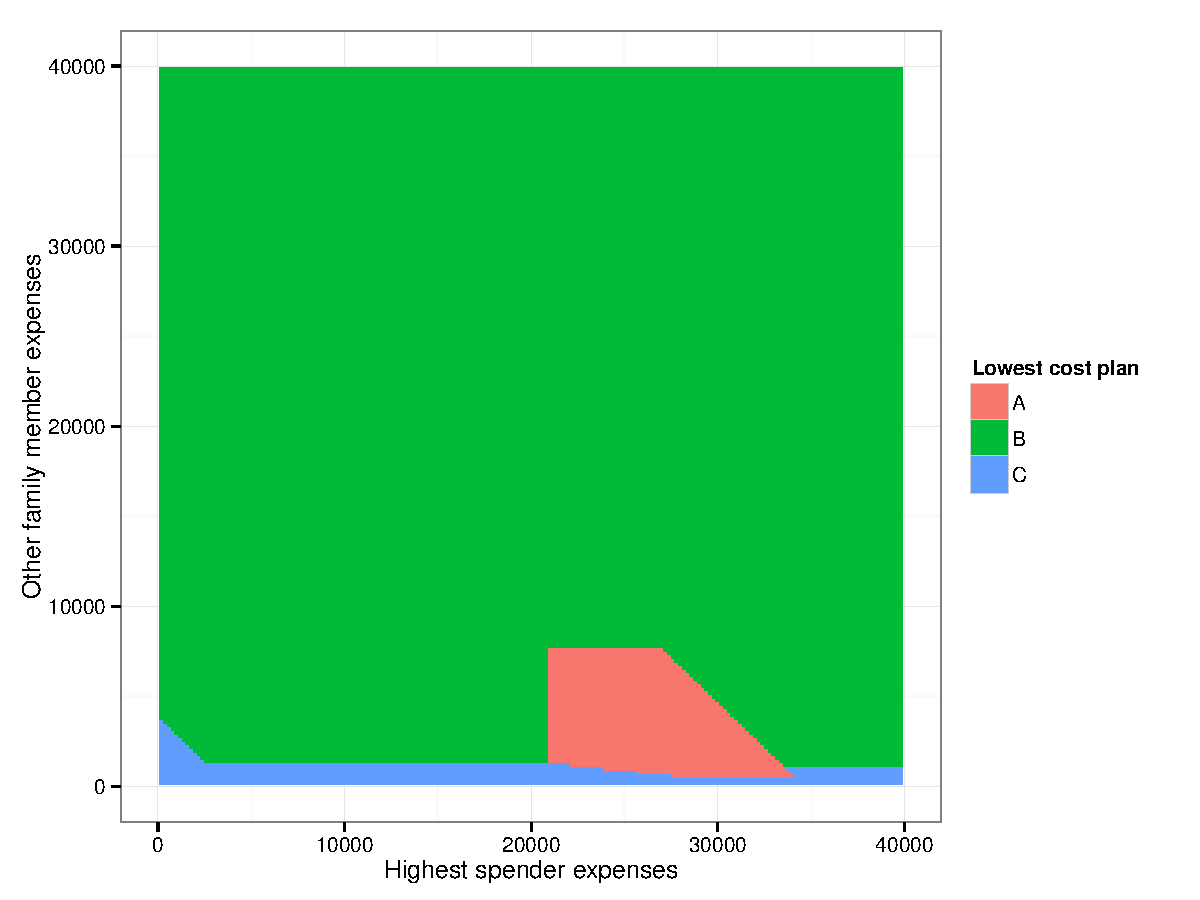
\includegraphics[height=5.5cm]{./img/ins-cost-map.pdf}
\end{center}
\end{frame}

\begin{frame}[fragile,label=sec-22]{Is there a better way?}
 \begin{itemize}
\item \texttt{shiny}, obviously!
\item Dynamic UI elements for \# of people on plan
\item "Interesting" \href{http://stackoverflow.com/questions/18116967/dealing-with-conditionals-in-a-better-manner-than-deeply-nested-ifelse-blocks}{algorithm} for dealing with complex criteria
\item Hosted internally at 3M  with \texttt{shiny-server}
\item Put an anonymized version on \href{https://www.shinyapps.io/}{shinyapps.io}
\end{itemize}
\end{frame}

\begin{frame}[label=sec-23]{Table of possible outcomes}
\begin{center}
\tiny
\begin{center}
\begin{tabular}{rrrrrrrl}
\toprule
ded\(_{\text{ind}}\) & oop\(_{\text{ind}}\) & ded\(_{\text{rem}}\) & oop\(_{\text{rem}}\) & ded\(_{\text{tot}}\) & oop\(_{\text{tot}}\) & bin & formula\\
\midrule
0 & 0 & 0 & 0 & 0 & 0 & 0 & exp\(_{\text{ind}}\) + exp\(_{\text{rem}}\)\\
1 & 0 & 0 & 0 & 0 & 0 & 1 & ded\(_{\text{ind}}\) + 0.1 (exp\(_{\text{ind}}\) - ded\(_{\text{ind}}\)) + exp\(_{\text{rem}}\)\\
0 & 0 & 1 & 0 & 0 & 0 & 4 & exp\(_{\text{ind}}\) + exp\(_{\text{rem}}\)\\
1 & 0 & 0 & 0 & 1 & 0 & 17 & ded\(_{\text{ind}}\) + 0.1 (exp\(_{\text{ind}}\) - ded\(_{\text{ind}}\)) + exp\(_{\text{rem}}\)\\
1 & 1 & 0 & 0 & 1 & 0 & 19 & oop\(_{\text{ind}}\) + exp\(_{\text{rem}}\)\\
0 & 0 & 1 & 0 & 1 & 0 & 20 & ded\(_{\text{tot}}\) + 0.1 (exp\(_{\text{ind}}\) + exp\(_{\text{rem}}\) - ded\(_{\text{tot}}\))\\
1 & 0 & 1 & 0 & 1 & 0 & 21 & ded\(_{\text{tot}}\) + 0.1 (exp\(_{\text{ind}}\) + exp\(_{\text{rem}}\) - ded\(_{\text{tot}}\))\\
1 & 1 & 1 & 0 & 1 & 0 & 23 & oop\(_{\text{ind}}\) + ded\(_{\text{ind}}\) + 0.1 (exp\(_{\text{rem}}\) - ded\(_{\text{ind}}\))\\
1 & 0 & 1 & 1 & 1 & 0 & 29 & ded\(_{\text{tot}}\) + 0.1 (exp\(_{\text{ind}}\) + exp\(_{\text{rem}}\) - ded\(_{\text{tot}}\))\\
1 & 1 & 0 & 0 & 1 & 1 & 51 & oop\(_{\text{ind}}\) + exp\(_{\text{rem}}\)\\
1 & 1 & 1 & 0 & 1 & 1 & 55 & oop\(_{\text{ind}}\) + ded\(_{\text{ind}}\) + 0.1 (exp\(_{\text{rem}}\) - ded\(_{\text{ind}}\))\\
1 & 0 & 1 & 1 & 1 & 1 & 61 & oop\(_{\text{tot}}\)\\
1 & 1 & 1 & 1 & 1 & 1 & 63 & oop\(_{\text{tot}}\)\\
\bottomrule
\end{tabular}
\end{center}
\normalsize
\end{center}
\end{frame}

\begin{frame}[fragile,label=sec-24]{Check against criteria; convert to binary}
 \scriptsize
\begin{verbatim}
  test_case <- c(rep(c(exp_ind, exp_rem, exp_ind + exp_rem),   # vector of predicted costs
                     each = 2))                                # for max vs. others

  test_case <- rbind(test_case, test_case, test_case)          # three sets for three plans
  
  limits <- cbind(compare$ded_ind, compare$exp_max_ind,        # criteria values
                  compare$ded_ind, compare$exp_max_ind, 
                  compare$ded_tot, compare$exp_max_tot)
  
  result <- cbind(compare[, c("ded_ind", "ded_tot", "oop_ind", # store cutoffs in result
                              "oop_tot", "prem", "hsa")],
                  exp_ind, exp_rem,
                  (test_case > limits) %*% (2^(0:5)))          # convert T/F to binary
\end{verbatim}
\normalsize
\end{frame}

\begin{frame}[fragile,label=sec-25]{Hacky function lookup}
 \tiny
\begin{verbatim}
map_funcs <- list(
  "0" = function(binary) { binary$exp_ind + binary$exp_rem }, 
  "1" = function(binary) { binary$ded_ind + (0.1* (binary$exp_ind - binary$ded_ind)) + binary$exp_rem }, 
  "4" = function(binary) { binary$exp_ind + binary$exp_rem }, 
  "16" = function(binary) { binary$ded_tot + (0.1 * (binary$exp_ind + binary$exp_rem - binary$ded_tot)) },
  "17" = function(binary) { binary$ded_ind + (0.1* (binary$exp_ind - binary$ded_ind)) + binary$exp_rem },
  "19" = function(binary) { binary$oop_ind + binary$exp_rem }, 
  "20" = function(binary) { binary$ded_tot + (0.1 * (binary$exp_ind + binary$exp_rem - binary$ded_tot)) }, 
  "21" = function(binary) { binary$ded_tot + (0.1 * (binary$exp_ind + binary$exp_rem - binary$ded_tot)) }, 
  "23" = function(binary) { binary$oop_ind + binary$ded_ind + (0.1 * (binary$exp_rem - binary$ded_ind)) },
  "28" = function(binary) { binary$ded_tot + (0.1 * (binary$exp_ind + binary$exp_rem - binary$ded_tot)) },
  "29" = function(binary) { binary$ded_tot + (0.1 * (binary$exp_ind + binary$exp_rem - binary$ded_tot)) },
  "48" = function(binary) { binary$oop_tot },   
  "51" = function(binary) { binary$oop_ind + binary$exp_rem }, 
  "55" = function(binary) { binary$oop_ind + binary$ded_ind + (0.1 * (binary$exp_rem - binary$ded_ind)) }, 
  "60" = function(binary) { binary$oop_tot }, 
  "61" = function(binary) { binary$oop_tot }, 
  "63" = function(binary) { binary$oop_tot }
)
\end{verbatim}
\normalsize
\end{frame}

\begin{frame}[label=sec-26]{}
\vfill
\begin{center}
'Nuff talk, let's take a \href{https://jwhendy.shinyapps.io/insurance-visualizer/}{look}!
\end{center}
\vfill
\end{frame}

\begin{frame}[fragile,label=sec-27]{So, why \emph{are} they smiling?}
 \begin{itemize}
\item Perhaps they were just playing with \texttt{shiny}!
\end{itemize}

\begin{center}
\includegraphics[height=5cm]{./img/choosing-insurance.jpg}
\end{center}

\vspace{-0.5cm}

\tiny
Image credit: \url{http://jtsfs.com/employee-benefits-2/group-health-insurance/}
\end{frame}

\begin{frame}[fragile,label=sec-28]{Sharing \texttt{shiny} apps}
 \begin{itemize}
\item tar/zip all files, send, have user run locally
\item Install \href{http://www.rstudio.com/shiny/server/}{shiny-server} on local machine

\item Request account on \emph{new} RStudio server \href{https://www.shinyapps.io/admin/#/signup}{here}
\begin{itemize}
\item Create apps locally, then follow setup \href{https://github.com/rstudio/shinyapps/blob/master/guide/guide.md}{instructions}
\item When satisfied, just run \texttt{deployApp()}!
\item App goes live at \url{http://uname.shinyapps.io/appName/}
\end{itemize}
\end{itemize}
\end{frame}

\begin{frame}[fragile,label=sec-29]{References}
 \begin{itemize}
\item \href{http://shiny.rstudio.com/tutorial/}{Getting started} with \texttt{shiny}
\item \texttt{shiny} \href{https://groups.google.com/forum/#!forum/shiny-discuss}{mailing list}
\item RStudio server account \href{https://shinyapps.io/}{request}
\item \href{http://stackoverflow.com/questions/19130455/create-dynamic-number-of-input-elements-with-r-shiny}{SO question} on creating dymanic input elements
\item \href{http://stackoverflow.com/questions/17683933/set-global-object-in-shiny}{SO question} on global variables (not intuitive!)
\item \href{http://stackoverflow.com/questions/17838709/scale-and-size-of-plot-in-rstudio-shiny}{SO question} on sizing plots in \texttt{shiny}
\item \href{http://stackoverflow.com/questions/17958730/faceting-a-set-of-contour-plots-in-ggplot-r}{SO question} that solved my contour plot issue; repaid with \texttt{shiny} example
\end{itemize}
\end{frame}

\begin{frame}[label=sec-30]{Apps in this presentation}
\begin{itemize}
\item \href{https://jwhendy.shinyapps.io/transpo-exploration/}{Transpo exploration}
\item \href{http://spark.rstudio.com/jwhendy/interactive-contour/}{Interactive contour}
\item \href{https://jwhendy.shinyapps.io/shiny-rcharts/}{rCharts example}
\item \href{http://spark.rstudio.com/jwhendy/insurance-visualizer/}{Benefit analysis}
\item Everything's also on \href{https://github.com/jwhendy/devFest-shiny}{github}!
\end{itemize}
\end{frame}
\begin{frame}[label=sec-31]{Tools}
Presentation made entirely with open source software!

\begin{center}
\begin{center}
\begin{tabular}{lllll}
\includegraphics[height=1.5cm]{./img/emacs.png} & \includegraphics[height=1.5cm]{./img/org-mode.png} & \includegraphics[height=1.5cm]{./img/r.png} & \includegraphics[height=1.5cm]{./img/r-studio.png} & \includegraphics[height=1.5cm]{./img/arch.png}\\
\end{tabular}
\end{center}
\end{center}

\begin{itemize}
\item \href{http://www.gnu.org/software/emacs/}{Emacs} and \href{http://orgmode.org/}{Org-mode} for reproducible code environment
\item \href{http://www.latex-project.org/}{\LaTeX} / \href{http://www.ctan.org/tex-archive/macros/latex/contrib/beamer/}{Beamer} for typesetting
\item \href{http://blog.barisione.org/2007-09/torino-a-pretty-theme-for-latex-beamer/}{Torino} Beamer theme so that it wasn't obvious I was using Beamer
\end{itemize}
\end{frame}

\begin{frame}[label=sec-32]{}
\LARGE
\begin{center}
Questions?

\vspace{1.5cm}

\normalsize
Come say "Hi" at the \href{http://www.meetup.com/twincitiesrug/}{TC R Users Group} to learn more :)
\end{center}
\end{frame}
% Emacs 24.4.1 (Org mode 8.3beta)
\end{document}
